\FloatBarrier
\section{Supporting Certificate and Moment Proofs}
\label{sec:theory-proofs}

\FloatBarrier
\subsection{Box Optimality}
\label{app:box-optimality}
\begin{proof}[Proof of \cref{thm:box-optimality}]
For the minimum, choose $m_{bj}=m^-_{bj}$ and $z_b=l_b$ if
$\nu_{bj}-c\ge0$, or $z_b=u_b$ otherwise. These simultaneous admissible
choices minimize every summand in \cref{eq:residual-identity}. Opposite mass
endpoints and $m_{bj}=m^+_{bj}$ attain the maximum. The matching inequalities
are \cref{eq:residual-enclosure}.
\end{proof}

\FloatBarrier
\subsection{The Row-Sum Quadratic Bound}
\label{app:quadratic-witness}
\begin{proof}[Proof of \cref{lem:quadratic-witness}]
The inequality $|u_a u_k|\le(u_a^2+u_k^2)/2$ and symmetry give
\begin{equation*}
 \begin{aligned}
 |u^TFu|&\le\frac12\sum_{a,k}|F_{ak}|(u_a^2+u_k^2)\\
 &=\sum_a u_a^2\sum_k|F_{ak}|\le\eta\sum_a u_a^2.
 \end{aligned}
\end{equation*}
No numerical eigendecomposition is needed.
\end{proof}

\FloatBarrier
\subsection{The Sharp Exponential Majorant}
\label{app:sharp-remainder}
\begin{proof}[Proof of \cref{lem:sharp-remainder}]
If $\rho=0$, then $t=0$. Otherwise absolute convergence of the exponential
series yields
\begin{equation*}
 \left|\sum_{n\ge3}\frac{t^n}{n!}\right|
 \le t^2\sum_{n\ge3}\frac{\rho^{n-2}}{n!}
 =\kappa(\rho)t^2.
\end{equation*}
Equality at $t=\rho>0$ forces every uniform coefficient to be at least
$\kappa(\rho)$. Substituting $n=m+3$ and using $(m+3)!\ge6m!$ gives
\begin{equation*}
 \kappa(\rho)=\sum_{m\ge0}\frac{\rho^{m+1}}{(m+3)!}
 \le\frac{\rho}{6}\sum_{m\ge0}\frac{\rho^m}{m!}.
\end{equation*}
For $\rho>0$, terms with $m\ge1$ make the inequality strict.
\end{proof}

\FloatBarrier
\subsection{Full-Score Enclosure from Signed Moments}
\label{app:full-score-enclosures}
\begin{proof}[Proof of \cref{thm:full-score-enclosures}]
Centering gives $\operatorname{mean}(t_i)=0$,
$\operatorname{mean}(t_i^2)=\sigma_b^2$, and
$\operatorname{mean}(x_{ij})=0$. Writing
$r_i=e^{t_i}-1-t_i-t_i^2/2$, \cref{lem:sharp-remainder} gives
$\operatorname{mean}|r_i|\le\tau_b$. Thus the projected mass lies in
$w_b[A_b-\tau_b,A_b+\tau_b]$. Jensen's inequality also bounds it below by
$w_b$, proving \cref{eq:projected-mass}.

The projected centered numerator equals
\begin{equation*}
 w_b\left[(C_b^Tu)_j+\tfrac12u^TH_{bj}u+
 \operatorname{mean}(r_i x_{ij})\right].
\end{equation*}
Apply \cref{lem:quadratic-witness} to $H_{bj}-D_{bj}$ and use
$|\operatorname{mean}(r_i x_{ij})|\le\tau_bR_{bj}$ to obtain
\cref{eq:projected-numerator}.

Restoring discarded coordinates multiplies each positive projected weight by
$e^{e_i}\in[e^{-\epsilon_b},e^{\epsilon_b}]$, proving \cref{eq:full-mass}.
Since $|e^{e_i}-1|\le e^{\epsilon_b}-1$, the centered numerator changes by
at most
\begin{equation*}
 \begin{aligned}
 &(e^{\epsilon_b}-1)R_{bj}\sum_{i\in b}e^{a_b-s+t_i}\\
 &\qquad\le(e^{\epsilon_b}-1)\widetilde u_bR_{bj}.
 \end{aligned}
\end{equation*}
Adding this perturbation proves \cref{eq:full-numerator}.
\end{proof}

\FloatBarrier
\subsection{Exact Polygon Support}
\label{app:polygon-support}
The rational optimizer enumerates polygon vertices. Candidate masses are
$l_b,u_b$ and $m^-_{bj}/s,m^+_{bj}/s$ for each nonzero
$s\in\{p_{bj},q_{bj}\}$. At a feasible mass $z$, the centered endpoints are
$\max(m^-_{bj},p_{bj}z)$ and $\min(m^+_{bj},q_{bj}z)$.
These cover intersections of vertical, horizontal, and sloping boundaries.
Distinct sloping lines meet at $z=0$, necessarily a mass endpoint if feasible
under $l_b\ge0$; coincident lines and degenerate segments add no candidates.
A linear objective attains its extrema at these vertices. Empty candidate
sets indicate inconsistent metadata and are rejected. The number of rational
operations is constant per block/channel; their bit cost is not.

\FloatBarrier
\subsection{Boundary Geometry}
\label{app:boundary-geometry}
\begin{example}\label{ex:boundary-geometry}
Two blocks with centers $0,2$, masses in $[1,2]$, and zero centered numerators
have output range $[2/3,4/3]$. Boundary signs certify $(0.6,1.4)$. A symmetric
residual bound about $1$ using midpoint masses has radius $0.5$ and fails.
This is a strict improvement in this example, not a dominance claim over
every correlated certificate.
\end{example}

\begin{figure}[!htbp]
 \centering
 % Native vector fragment. Required: tikz; arrows.meta; cmk{blue,orange,green,gray}.
% Exact witness: nu=(0,2), z_1,z_2 in [1,2], m_1=m_2=0.
% On 1/4 <= c <= 7/4, L(c)=2-3c and U(c)=4-3c.
\begin{tikzpicture}[font=\small, line cap=round, line join=round,
  >=Stealth, every node/.style={inner sep=2pt}]
  \path[use as bounding box] (-0.65,-0.9) rectangle (15.3,6.2);
  \node[anchor=west,font=\small\bfseries] at (-0.3,5.95)
    {(a) Exact boundary residuals};
  % x = 4(c-1/4); y = 3 + 0.7 residual.
  \fill[cmkblue!9] (0,3.875)--(6,0.725)--(6,2.125)--(0,5.275)--cycle;
  \draw[cmkgray!55,thin] (0,3)--(6.2,3);
  \draw[cmkgreen!65,densely dotted] (1.4,0.35)--(1.4,5.35);
  \draw[cmkgreen!65,densely dotted] (4.6,0.35)--(4.6,5.35);
  \draw[cmkblue,thick] (0,3.875)--(6,0.725);
  \draw[cmkorange,thick] (0,5.275)--(6,2.125);
  \node[anchor=west,text=cmkorange,fill=white] at (3.8,4.75)
    {$\mathcal U(c)=4-3c$};
  \node[anchor=west,text=cmkblue,fill=white] at (0.1,1.65)
    {$\mathcal L(c)=2-3c$};
  \fill[cmkgreen] (1.4,3.14) circle (2.4pt);
  \fill[cmkgreen] (4.6,2.86) circle (2.4pt);
  \draw[->] (0,0.35)--(6.25,0.35) node[anchor=west] {$c$};
  \draw[->] (0,0.35)--(0,5.5);
  \node[anchor=south west] at (0.1,5.35) {$N-cZ$};
  \foreach \x/\lab in {0/0.25,1.4/0.6,3/1,4.6/1.4,6/1.75} {
    \draw (\x,0.35)--(\x,0.27);
    \node[anchor=north,font=\footnotesize] at (\x,0.24) {$\lab$};
  }
  \foreach \y/\lab in {0.9/-3,1.6/-2,2.3/-1,3/0,3.7/1,4.4/2,5.1/3} {
    \draw (0,\y)--(-0.07,\y);
    \node[anchor=east,font=\footnotesize] at (-0.09,\y) {$\lab$};
  }
  \node[anchor=north,align=center,text=cmkgreen,font=\footnotesize]
    at (3,-0.25)
    {$\mathcal L(0.6)=0.2>0,\qquad\mathcal U(1.4)=-0.2<0$};
  \begin{scope}[xshift=8cm]
    \node[anchor=west,font=\small\bfseries] at (0,5.95)
      {(b) Output intervals};
    % x = 5.5(y-0.4); each row has its own descriptive label.
    \node[anchor=west] at (0,5.2) {Required open cell};
    \draw[cmkgreen,line width=2pt] (1.1,4.65)--(5.5,4.65);
    \foreach \x/\lab in {1.1/0.6,5.5/1.4} {
      \draw[cmkgreen,fill=white,thick] (\x,4.65) circle (2.5pt);
      \node[anchor=north,font=\footnotesize] at (\x,4.45) {$\lab$};
    }
    \node[anchor=west] at (0,3.65) {Exact attainable output range};
    \draw[cmkblue,line width=2pt] ({5.5*(2/3-0.4)},3.1)--({5.5*(4/3-0.4)},3.1);
    \foreach \x/\lab in {{5.5*(2/3-0.4)}/{2/3},{5.5*(4/3-0.4)}/{4/3}} {
      \fill[cmkblue] ({\x},3.1) circle (2.5pt);
      \node[anchor=north,font=\footnotesize] at ({\x},2.9) {$\lab$};
    }
    \node[anchor=west] at (0,2.1) {Symmetric residual bound};
    \draw[cmkorange,line width=2pt] (0.55,1.55)--(6.05,1.55);
    \foreach \x/\lab in {0.55/0.5,6.05/1.5} {
      \fill[cmkorange] (\x,1.55) circle (2.5pt);
      \node[anchor=north,font=\footnotesize] at (\x,1.35) {$\lab$};
    }
    \draw[->] (0,0.35)--(6.8,0.35);
    \foreach \x/\lab in {0/0.4,3.3/1,6.6/1.6} {
      \draw (\x,0.35)--(\x,0.27);
      \node[anchor=north,font=\footnotesize] at (\x,0.24) {$\lab$};
    }
    \node[anchor=north,font=\footnotesize] at (3.3,-0.25)
      {Normalized output $y=N/Z$};
  \end{scope}
\end{tikzpicture}

 \caption{Boundary residuals for \cref{ex:boundary-geometry}. The attained
 output range is closed; the certified open cell is illustrative, not a BF16
 rounding cell.}
 \label{fig:boundary-geometry}
\end{figure}

\FloatBarrier
\subsection{Joint Value Coupling}
\label{app:joint-coupling}
\begin{example}\label{ex:joint-coupling}
For $z\in[1,4]$, $m\in[1/2,3/2]$, and $-z/2\le m\le z/2$, consider
$m-z/4$. The box gives $[-1/2,5/4]$; the cone with the mass interval gives
$[-3,1]$. Intersecting these scalar bounds gives $[-1/2,1]$, whereas joint
optimization gives $[-1/2,3/4]$. This compares metadata geometry without
asserting token realizability of every vertex.
\end{example}

\FloatBarrier
\subsection{Margin and Refinement}
\label{app:margin-refinement}
The residual width separates mass and numerator uncertainty:
\begin{equation}
 \begin{aligned}
 W_j(c)&=\mathcal U_j(c)-\mathcal L_j(c)\\
 &=\sum_b\bigl[m^+_{bj}-m^-_{bj}+|\nu_{bj}-c|(u_b-l_b)\bigr].
 \end{aligned}
 \label{eq:residual-width}
\end{equation}
\begin{samepage}
\begin{proposition}[Margin versus uncertainty]\label{prop:margin-uncertainty}
For $a_j<y_j<b_j$, certification follows if
\begin{equation*}
 \begin{aligned}
 W_j(a_j)&<Z(y_j-a_j),\\
 W_j(b_j)&<Z(b_j-y_j).
 \end{aligned}
\end{equation*}
\end{proposition}
\end{samepage}
\begin{proof}
The lower endpoint is at least the true residual minus its enclosure width;
the upper endpoint is at most the true residual plus its width. The proposed
inequalities therefore give both strict signs.
\end{proof}
This explanatory condition requires unknown truth, so is not an executable
test. It explains difficult near-midpoint coordinates and prioritizing large
width contributions. If sound widths converge to zero and the output stays
strictly inside a fixed cell, that cell eventually passes. The bounded executor
does not assume convergence before fallback.

\FloatBarrier
\subsection{Diagonal Retention Need Not Produce Nested Intervals}
\label{app:diagonal-nonnesting}
Retaining the diagonal weakly reduces the row-sum witness but shifts the
approximation center, so the resulting intervals need not be nested.
For $H_{11}=9$, $H_{23}=H_{32}=10$, all other entries zero, and $u=(1,0,0)$,
both witnesses equal $10$. Retaining the diagonal changes $[-10,10]$ to
$9+[-10,10]$. Acceptance need not improve for every cell; both representations
are exposed by the implementation.

\FloatBarrier
\subsection{Remainder and Projection Growth}
\label{app:remainder-growth}
\Cref{fig:remainder-mechanism} compares the sharp remainder coefficient with
the Lagrange bound and isolates the separate cost of discarded-score variation.
\begin{figure}[!htbp]
 \centering
 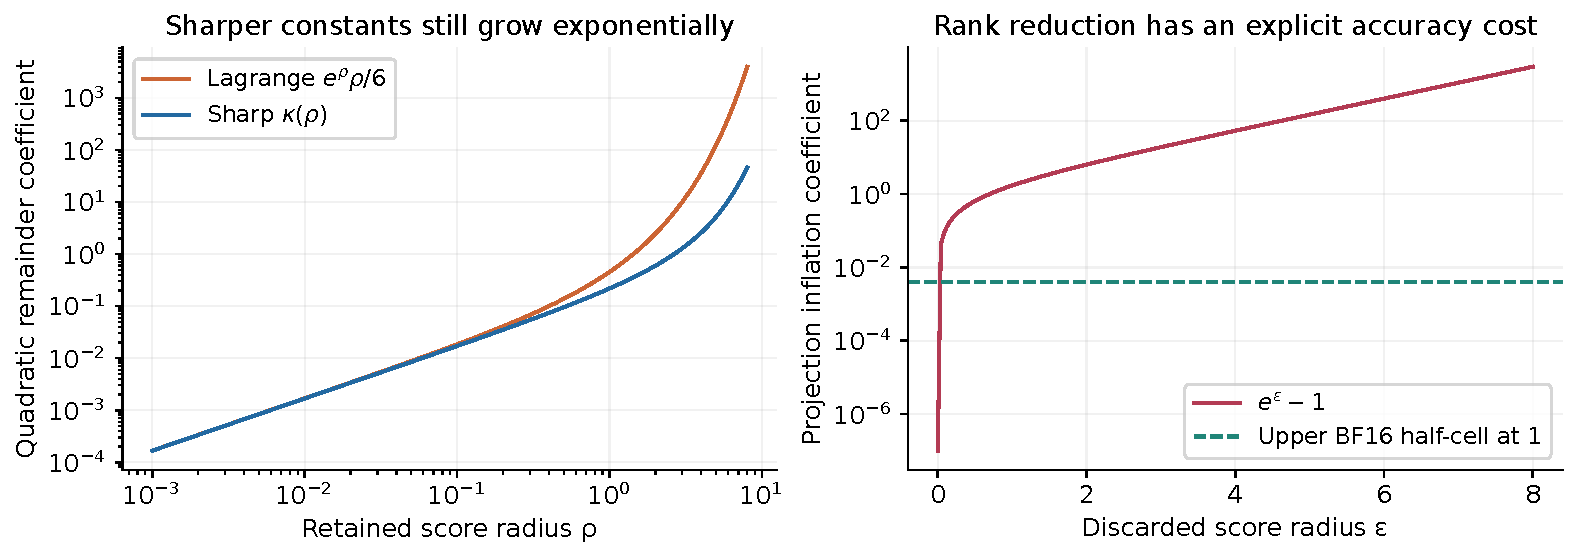
\includegraphics[width=\textwidth]{figures/remainder_mechanism.pdf}
 \caption{The sharp coefficient improves the Lagrange constant but still
 grows exponentially. Discarded scores impose a separate exponential cost.
 The BF16 line is a unit-scale guide, not a sufficient certificate.}
 \label{fig:remainder-mechanism}
\end{figure}

\FloatBarrier
